% !TEX root = handbook-physics.tex
%!TEX TS-program = pdflatex
%!TEX encoding = UTF-8 Unicode


\chapter{Newton's Laws}
\label{ch-02}

\section{Newton's First Law. Inertial Frames of Reference}
\label{sec-2.1}
\subsection{}\label{2.1.1} As the \emph{first law of dynamics} Newton took a law that had already been established by Galileo: a particle persistsing its state of rest or uniform motion in a straight line until the action of other bodies compel it to change that state.

Newton’s first law indicates that no external action is required to maintain a state of rest or of uniform motion in a straight line. This manifests a special dynamic property of bodies, called their \emph{inertia}. Newton’s first law is consequently called the \emph{law of inertia}, and the motion of a body not subject to the action of other bodies is said to be \emph{inertial motion}. 

\subsection{}\label{2.1.2}Mechanical motion is relative: its nature may differ for different frames of reference \ssect{1.2.1} that are moving in relation to each other. An astronaut, for instance, on board a man-made satellite orbiting the earth, may be at rest in a reference frame fixed in the satellite. At the same time, he is travelling together with the satellite with respect to the earth along an elliptic or­bit, i.e. not with uniform motion and not in a straight line. It is thus obvious that Newton’s first law does not hold for any frame of reference. A ball, for example, lying on the smooth floor of a stateroom in a ship travelling with uniform motion at sea in a straight line, may suddenly start moving along the floor without being subject to the action of any other bodies. This will occur when the velocity of the ship, i.e. its speed and/or direction, begins to change.

A frame of reference with respect to which a particle, not sub­ject to external action, remains at rest or moves uniformly in a straight line is called an \emph{inertial frame of reference}. The content of Newton’s first law reduces, in essence, to two statements: in the first place, that all material bodies possess the property of inertia, and secondly, that inertial reference frames exist.


\subsection{}\label{2.1.3}Any two inertial reference frames can move only with translational motion with respect to each other, and only uniformly in a straight line. It has been experimentally established that the \emph{heliocentric frame of reference} is practically inertial. The origin of its coordinate system is located at the centre of mass \ssect{2.3.3} of the solar system (approximately at the centre of the sun) and the three axes extend in the directions of three dis­tant stars selected, for example, so that these coordinate axes are mutually perpendicular.

A \emph{laboratory frame of reference}, whose coordinate axes are rigidly fixed in the earth, is noninertial chiefly owing to the earth’s diurnal (daily) rotation. But the earth rotates so slowly that the maximum normal acceleration \ssect{1.4.6} of points on its sur­face due to diurnal rotation does not exceed \SI{0.034}{\meter\per\second\squared}. There­fore, in the great majority of practical problems, the laboratory reference frame can be regarded as being approximately iner­tial.

\subsection{}\label{2.1.4} Inertial reference frames are of prime importance in all branches of physics, not only mechanics. This is due to the fact that according to Einstein’s principle of relativity \ssect{5.1.2} the mathematical expression of any physical law should have the same form in ail inertial reference frames. Hence, in the following we shall make use of only inertial frames of reference, without stipulation each time. The laws of motion of a particle with respect to a noninertial reference frame is dealt with in \textcolor{IndianRed}{Chapter~\ref{ch-07}}.

%\begin{equation*}%
%\vb{r}= x \vb{i} + y \vb{j} + z \vb{k}
%\end{equation*}
%
%\begin{wrapfigure}{r}{0.5\linewidth}
%\centering
%%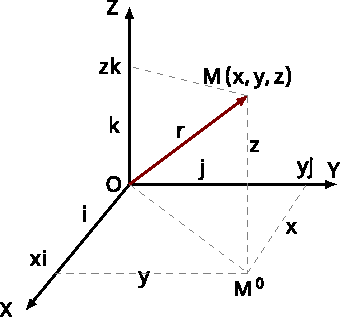
\includegraphics{figs/ch-01/fig-01-01.pdf}
%% !TEX root = ../../handbook-physics.tex
%!TEX TS-program = pdflatex
%!TEX encoding = UTF-8 Unicode


%\documentclass{article}
%\usepackage[svgnames]{xcolor}
%\usepackage{tikz}
%\usepackage{amsmath}
%\usepackage{physics}
%
%\begin{document}
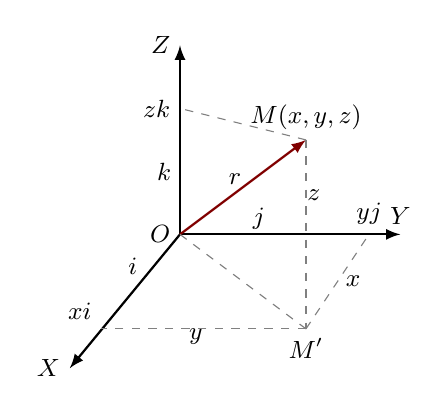
\begin{tikzpicture}[scale=0.4,font=\small]
		\node [] (0) at (0, 6){};
		\node [] (1) at (0, 0) {};
		\node [] (2) at (-3.5, -4.25) {};
		\node [] (3) at (7, 0) {};
		\node [] (4) at (4, 3) {};
		\node [] (5) at (4, -3) {};
		\node [] (6) at (0, 4) {};
		\node [] (7) at (6, 0) {};
		\node [] (8) at (-2.5, -3) {};
		\node [] (9) at (1.75, 1.75) {};
		\node [] (10) at (1.75, 1.75) {$\vb{r}$};
		\node [] (11) at (-0.5, 2) {$\vb{k}$};
		\node [] (12) at (-1.5, -1) {$\vb{i}$};
		\node [] (13) at (2.5, 0.5) {$\vb{j}$};
		\node [] (14) at (0.5, -3.25) {};
		\node [] (15) at (5.5, -1.5) {};
		\node [] (16) at (4.25, 1.25) {};
		\node [] (18) at (5.5, -1.5) {$x$};
		\node [] (19) at (0.5, -3.25) {};
		\node [] (20) at (0.5, -3.25) {$y$};
		\node [] (21) at (4.25, 1.25) {$z$};
		\draw [thick,latex-](0.center) to (1.center);
		\draw [thick,-latex](1.center) to (2.center);
		\draw [thick,-latex](1.center) to (3.center);
		\draw [thick,-latex,Maroon](1.center) to (4.center);
		\draw [dashed,gray](1.center) to (5.center);
		\draw [dashed,gray](4.center) to (6.center);
		\draw [dashed,gray](4.center) to (5.center);
		\draw [dashed,gray](5.center) to (7.center);
		\draw [dashed,gray](5.center) to (8.center);
		\node [left] at (0,0) {$O$};
		\node [left] at (0,6) {$Z$};
		\node [left] at (-3.5, -4.25) {$X$};
		\node [above] at (7, 0) {$Y$};
		\node [above] at (4, 3) {$M (x,y,z)$};
		\node [below] at (4, -3) {$M'$};
		\node [left] at (0,4) {$z\vb{k}$};
		\node [above] at (6,0) {$y\vb{j}$};
		\node [above left] at (-2.5, -3) {$x\vb{i}$};
\end{tikzpicture}
%\end{document}
%%  \vspace{-13pt}
%\caption{Cartesian system of coordinates.}
%\label{fig-01-01}
%\end{wrapfigure}
%
